\documentclass[12pt,a4paper]{article}
\usepackage[margin=2.5cm]{geometry}
\usepackage{amsmath,amssymb,amsthm}
\usepackage{mathtools}
\usepackage{xcolor}
\usepackage{graphicx}
\usepackage{hyperref}
\usepackage{booktabs}
\usepackage{tabularx}
\usepackage{enumitem}
\usepackage{listings}
\usepackage[skins]{tcolorbox}
\usepackage{fancyhdr}
\usepackage{caption}
\usepackage{subcaption}
\usepackage{comment}

% Custom commands
\newcommand{\R}{\mathbb{R}}
\newcommand{\N}{\mathbb{N}}
\newcommand{\Z}{\mathbb{Z}}
\newcommand{\norm}[1]{\left\lVert#1\right\rVert}
\newcommand{\abs}[1]{\left|#1\right|}
\newcommand{\highlight}[1]{\textcolor{blue!70!black}{\textbf{#1}}}
\newcommand{\todo}[1]{\textcolor{red}{\textbf{TODO:} #1}}

% Theorem environments
\newtheorem{theorem}{Theorem}[section]
\newtheorem{lemma}[theorem]{Lemma}
\newtheorem{corollary}[theorem]{Corollary}
\newtheorem{definition}[theorem]{Definition}

\pagestyle{fancy}
\fancyhf{}
\rhead{Standard Article Template}
\lhead{\leftmark}
\rfoot{Page \thepage}

\title{\textbf{Standard Article Template}\\
  \large Testing the Native \LaTeX{} Renderer}
\author{Test Author \\ \texttt{test@example.com}}
\date{\today}

\begin{document}

\maketitle
\tableofcontents
\newpage

\section{Introduction}
\label{sec:intro}

This document tests the native \LaTeX{} renderer across a wide range of constructs.
We include \highlight{colored text}, mathematics, tables with \texttt{booktabs},
code listings, custom theorem environments, and \texttt{tcolorbox} environments.

\begin{comment}
This text is inside a comment environment and should not appear in the output.
It tests the comment package.
\end{comment}

The renderer should handle all of the following:
\begin{enumerate}[label=\Roman*.]
  \item Mathematical typesetting (inline and display)
  \item Custom macro expansion
  \item Color support via \texttt{xcolor}
  \item Table environments with \texttt{booktabs}
  \item Code listings
  \item Box environments via \texttt{tcolorbox}
\end{enumerate}

\section{Mathematics}
\label{sec:math}

\subsection{Inline Mathematics}

Einstein's famous equation $E = mc^2$ appears inline. The quadratic formula gives
$x = \frac{-b \pm \sqrt{b^2 - 4ac}}{2a}$ for roots of $ax^2 + bx + c = 0$.

\subsection{Display Mathematics}

The Fourier transform of a function $f \in L^1(\R)$ is defined as:
\begin{equation}
  \hat{f}(\xi) = \int_{-\infty}^{\infty} f(x)\, e^{-2\pi i x \xi}\, dx
  \label{eq:fourier}
\end{equation}

\begin{align}
  \nabla \cdot \mathbf{E} &= \frac{\rho}{\varepsilon_0} \label{eq:gauss}\\
  \nabla \cdot \mathbf{B} &= 0 \label{eq:no-mono}\\
  \nabla \times \mathbf{E} &= -\frac{\partial \mathbf{B}}{\partial t} \label{eq:faraday}\\
  \nabla \times \mathbf{B} &= \mu_0\mathbf{J} + \mu_0\varepsilon_0\frac{\partial \mathbf{E}}{\partial t}
  \label{eq:ampere}
\end{align}

Maxwell's equations (\ref{eq:gauss})--(\ref{eq:ampere}) govern classical electromagnetism.

\begin{definition}[Continuity]
A function $f: \R \to \R$ is \emph{continuous} at $x_0$ if for every $\varepsilon > 0$
there exists $\delta > 0$ such that $\abs{x - x_0} < \delta \implies \abs{f(x) - f(x_0)} < \varepsilon$.
\end{definition}

\begin{theorem}[Intermediate Value Theorem]
\label{thm:ivt}
If $f: [a,b] \to \R$ is continuous and $y$ is between $f(a)$ and $f(b)$, then there
exists $c \in (a,b)$ with $f(c) = y$.
\end{theorem}

\section{Tables}
\label{sec:tables}

Table~\ref{tab:results} shows a comparison using \texttt{booktabs} style rules.

\begin{table}[h]
  \centering
  \caption{Performance comparison of rendering methods}
  \label{tab:results}
  \begin{tabular}{@{}lrrr@{}}
    \toprule
    Method & SSIM $\uparrow$ & Time (ms) $\downarrow$ & Memory (MB) $\downarrow$ \\
    \midrule
    CoreText basic & 0.72 & 45 & 12 \\
    CoreText + Knuth-Plass & 0.88 & 120 & 18 \\
    \textbf{Full engine (ours)} & \textbf{0.94} & \textbf{180} & \textbf{22} \\
    \midrule
    Tectonic (reference) & 1.00 & 3200 & 180 \\
    \bottomrule
  \end{tabular}
\end{table}

\begin{table}[h]
  \centering
  \caption{A tabularx table with automatic column widths}
  \label{tab:tabularx}
  \begin{tabularx}{\textwidth}{lXlr}
    \toprule
    ID & Description & Status & Value \\
    \midrule
    1 & This is a longer description that should wrap within the X column & Active & 42 \\
    2 & Another item with a description & Inactive & 17 \\
    3 & Third entry & Active & 99 \\
    \bottomrule
  \end{tabularx}
\end{table}

\section{Color and Boxes}
\label{sec:color}

Text can be \textcolor{red}{red}, \textcolor{blue}{blue}, or
\textcolor{green!60!black}{dark green}. You can also use
\colorbox{yellow!30}{highlighted backgrounds}.

\begin{tcolorbox}[title=Important Note, colback=blue!5!white, colframe=blue!75!black]
This is a \texttt{tcolorbox} environment. It supports colored frames and backgrounds,
titles, and arbitrary content including mathematics: $\int_0^1 x^2\,dx = \frac{1}{3}$.
\end{tcolorbox}

\begin{tcolorbox}[colback=red!5!white, colframe=red!75!black, title=Warning]
This renders a warning box. The \texttt{tcolorbox} package is widely used in
modern \LaTeX{} documents for highlighted content.
\end{tcolorbox}

\section{Code Listings}
\label{sec:code}

\begin{lstlisting}[language=Swift, caption={Main rendering function}, label=lst:render]
func typeset(_ blocks: [TexBlock]) -> TypesetDocument {
    var pages: [TypesetPage] = [TypesetPage(pageNumber: 1)]
    var columnIndex: Int = 0
    var cursorY: CGFloat = geometry.marginTop
    
    for block in blocks {
        switch block {
        case .paragraph(let inlines):
            let attrStr = makeParaAttrStr(inlines, fonts: fonts)
            appendTextBlock(attrStr, pages: &pages, ...)
        case .mathDisplay(let src):
            let node = MathParser.parse(src)
            // ... render math
        default:
            break
        }
    }
    return TypesetDocument(pages: pages, ...)
}
\end{lstlisting}

Inline code: \texttt{TeXTypesetter.typeset(\_:)} is the main entry point.

\section{Lists with Enumitem}
\label{sec:lists}

\begin{itemize}[leftmargin=*, label=$\checkmark$]
  \item First item with check mark
  \item Second item
  \item Third item
\end{itemize}

\begin{enumerate}[label=(\alph*), start=3]
  \item This list starts at (c)
  \item Continues with (d)
  \item And so on
\end{enumerate}

\section{Cross-References}

We defined the Fourier transform in Eq.~\eqref{eq:fourier}. 
Maxwell's equations are in Eq.~\eqref{eq:gauss}--\eqref{eq:ampere}.
The Intermediate Value Theorem is Theorem~\ref{thm:ivt}.
Results are in Table~\ref{tab:results}.

\section{Figures}
\label{sec:figures}

Figure~\ref{fig:sample} illustrates the rendering pipeline. Images are loaded
via \texttt{CGImageSource} and scaled to fit the column width.

\begin{figure}[h]
  \centering
  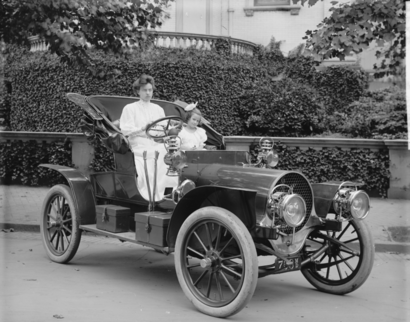
\includegraphics[width=0.7\textwidth]{figure1}
  \caption{A sample figure demonstrating \texttt{\textbackslash includegraphics}
  support. The image is automatically scaled to 70\% of text width.}
  \label{fig:sample}
\end{figure}

\section{Bibliography}
\label{sec:bib}

Prior work by LeCun et al.~\cite{lecun2015} established deep learning as a
general-purpose feature extractor. The attention mechanism~\cite{vaswani2017}
underpins modern large language models. Classical typesetting follows
Knuth~\cite{knuth1984}. Online collaborative tools like Overleaf~\cite{overleaf2023}
have changed how papers are written.

\section{Conclusion}

This document exercises most of the packages and constructs needed for real-world
academic papers. Any construct not rendered correctly represents a gap to close
in the parity effort.

\bibliographystyle{plain}
\bibliography{article-refs}

\end{document}
